%!TEX root = ../dokumentation.tex

\chapter{Implementation}
\label{chap:implementation}

Dieses Kapitel befasst sich mit der Implementation der Künstlichen Intelligenz. Dazu gehört zunächst die Implementation
der Spiellogik von Othello, die Implementation der eigentlichen Künstlichen Intelligenz unter Anwendung der im
\autoref{chap:theorie} genannten Techniken, außerdem mehrere Experimente zur Bestimmung der optimalen Parameter, sowie eine Grafische
Benutzeroberfläche zum Testen der Künstlichen Intelligenz. Die Implementation dieser Komponenten erfolgt in der
Programmiersprache Python unter Verwendung von Jupyter Notebooks. 

\hypertarget{spiellogik-othello_game.ipynb}{%
\section{Spiellogik
(othello\_game.ipynb)}\label{spiellogik-othello_game.ipynb}}

\label{sec:gamelogic} \ifx false

\begin{lstlisting}[language=Python]
%%HTML
<style>
.container { width:100% }
</style>
\end{lstlisting}

\fi Im Folgenden ist die Spielelogik des Spiels Othello implementiert.
Dazu gehört die Implementierung aller im \autoref{sec:spieltheorie}
genannten Aspekte, wie zum Beispiel die Erzeugung eines Startzustands,
sowie die Bestimmung und Durchführung von Spielzügen ausgehend von einem
Spielzustand.

\hypertarget{importieren-der-externen-abhuxe4ngigkeiten}{%
\subsection{Importieren der externen
Abhängigkeiten}\label{importieren-der-externen-abhuxe4ngigkeiten}}

Die Implementierung stützt sich für bessere Performanz auf die
Python-Bibliothek \passthrough{\lstinline!numpy!}, welche unter anderem
homogene Felder und Matrizen implementiert. Eine solche Matrix wird als
interne Repräsentation des Othello Spielfelds genutzt. Insbesondere
Operationen, die auf einen größeren Teil des Spielfelds zugreifen
müssen, können dadurch beschleunigt werden.

Für das Kopieren der Spielzustände wird das Modul
\passthrough{\lstinline!copy!} aus der Python Standardbibliothek
verwendet.

\begin{lstlisting}[language=Python]
import numpy as np
import copy
\end{lstlisting}

\hypertarget{globale-konstanten}{%
\subsection{Globale Konstanten}\label{globale-konstanten}}

Im folgenden Abschnitt werden zunächst einige Konstanten definiert,
welche in der späteren Implementierung häufig genutzt werden.

Die Konstante \passthrough{\lstinline!BOARD\_SIZE!} gibt die Anzahl an
Zeilen und Spalten des quadratischen Othello Spielfelds an.
\passthrough{\lstinline!BOARD\_SIZE!} wird beispielsweise zur Iteration
über Zeilen und Spalten des Spielfeldes genutzt, sowie zur Überprüfung,
ob gegebene Koordinaten innerhalb des Spielfeldes liegen.

Die Konstanten \passthrough{\lstinline!BLACK!},
\passthrough{\lstinline!WHITE!} und \passthrough{\lstinline!NONE!}
werden auf die Zahlenwerte -1, 1 und 0 abgebildet und werden für mehrere
Zwecke genutzt:

\begin{enumerate}
\def\labelenumi{\arabic{enumi}.}
\tightlist
\item
  Repräsentation des Spielfeldes: Das Othello Spielbrett wird als
  \(8\times 8\) Matrix von Ganzzahlen definiert, welche jeweils einen
  der drei Werte annehmen können. Hierbei stehen die Werte
  \passthrough{\lstinline!BLACK!} und \passthrough{\lstinline!WHITE!}
  jeweils für einen Stein des jeweiligen Spielers, während
  \passthrough{\lstinline!NONE!} ein leeres Feld repräsentiert.
\item
  Repräsentation der Spieler: \passthrough{\lstinline!BLACK!} und
  \passthrough{\lstinline!WHITE!} werden zur Repräsentation eines
  Spielers genutzt. Beispielsweise enthält der Spielzustand eine
  Variable \passthrough{\lstinline!turn!}, die angibt, welcher Spieler
  am Zug ist.
\item
  Berechnung der Heuristiken: Die Werte \passthrough{\lstinline!BLACK!},
  \passthrough{\lstinline!WHITE!} und \passthrough{\lstinline!NONE!}
  sind so gewählt, dass sie sich für die Berechnung der Heuristiken
  eignen. Der in der \ac{KI} maximierende Spieler hat den positiven Wert
  1, während der minimierende Spieler durch den negativen Wert -1
  repräsentiert wird. Kein Spieler wird durch den Wert 0 dargestellt.
\end{enumerate}

\begin{lstlisting}[language=Python]
BOARD_SIZE = 8

BLACK = -1  # MINIMIZING PLAYER
WHITE =  1  # MAXIMIZING PLAYER
NONE  =  0  # NO PLAYER
\end{lstlisting}

\hypertarget{game-state}{%
\subsection{Game State}\label{game-state}}

Die Klasse \passthrough{\lstinline!GameState!} repäsentiert einen
Spielzustand von Othello. Dieser wird durch die im Folgenden genannten
Attribute beschrieben:

\begin{itemize}
\tightlist
\item
  Das Spielfeld \passthrough{\lstinline!board!}, welches durch eine
  zweidimensionale Numpy-Matrix repräsentiert wird, bei der jede Zelle
  die die Werte \passthrough{\lstinline!BLACK!},
  \passthrough{\lstinline!WHITE!} und \passthrough{\lstinline!NONE!}
  annehmen kann.
\item
  Den Spieler \passthrough{\lstinline!turn!}, der im Spielzustand am Zug
  ist. Zusätzlich enthält der Spielzustand weitere Informationen, die
  zur Verbesserung der Performanz genutzt werden.
\item
  Die im aktuellen Spielzustand möglichen Züge werden als Paare von
  Koordinaten in der Variable \passthrough{\lstinline!possible\_moves!}
  gespeichert. Ein Koordinatenpaar steht hierbei für das Setzen eines
  Spielsteins auf die entsprechende Stelle auf dem Spielfeld unter
  Anwendung der Othello Regeln. Diese Variable ist Teil von
  \passthrough{\lstinline!GameState!}, damit pro Spielzustand die
  möglichen Züge nicht mehrfach berechnet werden müssen.
\item
  Die Menge der freien Felder, die horizontal, vertikal oder diagonal an
  einen Stein angrenzen wird in der Variable
  \passthrough{\lstinline!frontier!} gespeichert. Beim Ermitteln der
  möglichen Züge kann dadurch die Performanz wesentlich gesteigert
  werden, da nur diese Menge und nicht das gesamte Spielfeld überprüft
  werden muss.
\item
  Die Anzahl an Spielsteinen auf dem Spielfeld wird in der Variable
  \passthrough{\lstinline!num\_pieces!} gehalten.
\item
  Ob der Spielzustand ein Endzustand ist, wird in der Variable
  \passthrough{\lstinline!game\_over!} gespeichert.
\item
  Die Koordinaten des letzten Spielzugs werden zur späteren
  Visualisierung in der \ac{GUI} in der Variable
  \passthrough{\lstinline!last\_move!} gespeichert.
\end{itemize}

Die zur Performance-Verbesserung genutzten Variablen werden im Laufe des
Spielverlaufs immer aktuell gehalten.

In dem Konstruktor \passthrough{\lstinline!\_\_init\_\_!} der Klasse
\passthrough{\lstinline!GameState!} wird ein neuer Spielzustand
entsprechend den Othello Spielregeln instanziiert, indem alle Variablen
entsprechend initialisiert werden.

Die Funktion \passthrough{\lstinline!\_\_lt\_\_!} ist implementiert,
damit auf \passthrough{\lstinline!GameState!}-Objekten der
Vergleichsoperator angewendet werden kann. Das ist nötig, damit in der
\ac{KI} Tupel sortiert werden können, die beispielsweise aus einer
Priorität und einen \passthrough{\lstinline!GameState!} bestehen. Da in
diesem Fall nur die Sortierung nach der Priorität wichtig ist, ist die
Implementierung von \passthrough{\lstinline!\_\_lt\_\_!} irrelevant.
Daher wird der Einfachkeit halber immer True zurückgegeben.

\begin{lstlisting}[language=Python]
class GameState:
    def __init__(self):
        self.board = np.zeros((BOARD_SIZE, BOARD_SIZE), dtype=np.int8)
        self.board[3, 3] = WHITE
        self.board[3, 4] = BLACK
        self.board[4, 3] = BLACK
        self.board[4, 4] = WHITE
        self.turn = BLACK
        self.possible_moves = [(2, 3), (3, 2), (4, 5), (5, 4)]
        self.frontier = {(2, 2), (2, 3), (2, 4), (2, 5),
                         (3, 2), (3, 5), (4, 2), (4, 5),
                         (5, 2), (5, 3), (5, 4), (5, 5)}
        self.num_pieces = 4
        self.game_over = False
        self.last_move = None

    def __lt__(self, other):
        return True
\end{lstlisting}

Die Liste \passthrough{\lstinline!directions!} enthält alle
horizontalen, vertikalen und diagonalen Richtungen auf dem Spielfeld als
Zwei-Tupel. Die beiden Zahlen stellen hierbei jeweils den Versatz in
Reihen- und Spaltenrichtung dar. Diese Liste wird später in mehreren
Funktionen genutzt.

\begin{lstlisting}[language=Python]
directions = [(-1,-1),(0,-1),(1,-1),(-1,0),(1,0),(-1,1),(0,1),(1,1)]
\end{lstlisting}

Die Exception \passthrough{\lstinline!InvalidMoveException!}, wird
später in der Funktion \passthrough{\lstinline!make\_move!} geworfen,
wenn ein ungültiger Spielzug gefordert wird. Dies dient der
Fehlerbehandlung.

\begin{lstlisting}[language=Python]
class InvalidMoveException(Exception):
    pass
\end{lstlisting}

Die Funktion \passthrough{\lstinline!can\_flip\_in\_dir!} überprüft für
ein Spielfeld \passthrough{\lstinline!board!} und den Spieler
\passthrough{\lstinline!player!}, ob beim Setzen eines Steins auf die
Position \passthrough{\lstinline!pos!} in die Richtung
\passthrough{\lstinline!direction!} nach den Regeln von Othello Steine
umgedreht werden können. Die Variable \passthrough{\lstinline!board!}
enthält das Spielfeld als Python-Liste, da einzelne Zugriffe so deutlich
schneller sind, als bei einem Numpy-Array.
\passthrough{\lstinline!can\_flip\_in\_dir!} gibt einen Wahrheitswert
zurück. Dabei bedeutet \passthrough{\lstinline!True!}, dass Steine
umgedreht werden können.

\begin{lstlisting}[language=Python]
def can_flip_in_dir(board, pos, direction, player):
    row, col = pos
    rowdelta, coldelta = direction
    current_row = row + rowdelta
    current_col = col + coldelta
    if not (0 <= current_row < 8 and 0 <= current_col < 8):
        return False
    if not board[current_row][current_col] == -player:
        return False
    current_row += rowdelta
    current_col += coldelta
    
    while True:
        if not (0 <= current_row < 8 and 0 <= current_col < 8):
            return False
        if board[current_row][current_col] == NONE:
            return False           
        if board[current_row][current_col] == player:
            return True
    
        current_row += rowdelta
        current_col += coldelta
\end{lstlisting}

Die Funktion \passthrough{\lstinline!is\_move\_valid!} überprüft für ein
gegebenes Spielfeld \passthrough{\lstinline!board!}, ob ein Zug auf die
Position \passthrough{\lstinline!pos!} für den Spieler
\passthrough{\lstinline!player!} möglich ist. Das Ergebnis wird als
Wahrheitswert zurückgegeben. \passthrough{\lstinline!board!} ist hier
ebenfalls eine Python-Liste, da der Zugriff auf einzelne Elemente
schneller ist, als bei einem Numpy-Array.

\begin{lstlisting}[language=Python]
def is_move_valid(board, pos, player):
    for direction in directions:
        if can_flip_in_dir(board, pos, direction, player):
            return True
    return False
\end{lstlisting}

\passthrough{\lstinline!get\_utility!} bestimmt für einen
Endspielzustand \passthrough{\lstinline!state!} den Gewinner des Spiels
anhand der Anzahl an Spielsteinen, die beide Spieler auf dem Spielfeld
haben. Gewinnt Weiß, so wird der Wert der Konstante
\passthrough{\lstinline!WHITE!} zurückgegeben. Gewinnt Schwarz, wird der
Wert der Konstante \passthrough{\lstinline!BLACK!} zurückgegeben. Bei
einem Unentschieden wird der Wert von \passthrough{\lstinline!NONE!}
zurückgegeben.

\begin{lstlisting}[language=Python]
def get_utility(state):
    black_disks = count_disks(state, BLACK)
    white_disks = count_disks(state, WHITE)
    if black_disks > white_disks:
        return BLACK
    if white_disks > black_disks:
        return WHITE
    else:
        return NONE
\end{lstlisting}

Die Funktion \passthrough{\lstinline!get\_possible\_moves!} bestimmt für
einen Spielzustand \passthrough{\lstinline!state!} und den Spieler
\passthrough{\lstinline!player!} alle möglichen Züge, die
\passthrough{\lstinline!player!} im Spielzustand
\passthrough{\lstinline!state!} machen kann. Die resultierenden Züge
werden als Liste von Koordinatenpaaren zurückgegeben. Für eine bessere
Performanz werden nur Felder aus der Menge
\passthrough{\lstinline!frontier!} als mögliche Züge betrachtet.

\begin{lstlisting}[language=Python]
def get_possible_moves(state, player):
    board = state.board.tolist()
    possible_moves = []
    for pos in state.frontier:
        if is_move_valid(board, pos, player):
            possible_moves.append(pos)
    return possible_moves
\end{lstlisting}

Die Funktion \passthrough{\lstinline!flip\_in\_dir!} dreht im
Spielzustand \passthrough{\lstinline!state!}, ausgehend von dem durch
\passthrough{\lstinline!pos!} angegebenen Feld, die für den Spieler
\passthrough{\lstinline!player!} gegnerischen Steine in die Richtung
\passthrough{\lstinline!direction!} um. Der eingegebene
\passthrough{\lstinline!state!} wird dabei modifiziert. Die Funktion hat
keinen Rückgabewert.

\begin{lstlisting}[language=Python]
def flip_in_dir(state, pos, direction, player):
    (row, col) = pos
    rowdelta, coldelta = direction
    current_row = row + rowdelta
    current_col = col + coldelta
    
    while state.board[current_row, current_col] == -player:
        state.board[(current_row, current_col)] = player
        current_row += rowdelta
        current_col += coldelta
\end{lstlisting}

\passthrough{\lstinline!update\_frontier!} wird nach jedem Zug
aufgerufen, um die Menge \passthrough{\lstinline!frontier!} des
Spielzustands \passthrough{\lstinline!state!} zu aktualisieren. Die
durch \passthrough{\lstinline!pos!} gegebene Koordinate wird entfernt,
während die Koordinaten aller leeren umliegenden Felder hinzugefügt
werden. Der Spielzustand \passthrough{\lstinline!state!} wird hierbei
direkt verändert und es wird kein Wert zurückgegeben.

\begin{lstlisting}[language=Python]
def update_frontier(state, pos):
    (row, col) = pos
    for current_row in range(row-1, row+2):
        if not 0 <= current_row < 8:
            continue
        for current_col in range(col-1, col+2):
            if not 0 <= current_col < 8:
                continue
            if state.board[current_row, current_col] == NONE:
                state.frontier.add((current_row, current_col))
    state.frontier.remove((row, col))
\end{lstlisting}

Die Funktion \passthrough{\lstinline!count\_disks!} zählt die Steine,
die der Spieler \passthrough{\lstinline!player!} im Spielzustand
\passthrough{\lstinline!state!} auf dem Spielfeld hat. Die resultierende
Anzahl wird von der Funktion zurückgegeben.

\begin{lstlisting}[language=Python]
def count_disks(state, player):
    return np.count_nonzero(state.board == player)
\end{lstlisting}

\passthrough{\lstinline!get\_player\_string!} konvertiert die
Zahlenrepräsentation des Spielers \passthrough{\lstinline!player!} in
den Namen des Spielers. Ist \passthrough{\lstinline!player == NONE!}, so
wird `Nobody' zurückgegeben.

\begin{lstlisting}[language=Python]
def get_player_string(player):
    return {BLACK: 'Black', WHITE: 'White', NONE: 'Nobody'}[player]
\end{lstlisting}

Die Funktion \passthrough{\lstinline!make\_move!} versucht auf einem
Spielzustand \passthrough{\lstinline!state!} einen Spielzug entsprechend
den Othello Regeln auszuführen. Der auszuführende Zug wird hierbei durch
den Parameter \passthrough{\lstinline!pos!} bestimmt, welcher die
Spielfeldkoordinaten des zu setzenden Steins als Zwei-Tupel angibt.

Zunächst wird überprüft, ob die Koordinate \passthrough{\lstinline!pos!}
in der Variable \passthrough{\lstinline!frontier!} enthalten ist. Ist
dies nicht der Fall, so kann die Funktion mit einer
\passthrough{\lstinline!InvalidMoveException!} abgebrochen werden, da
ein Spielstein nur auf ein leeres Feld gesetzt werden kann, welches an
einen Spielstein angrenzt. Hierbei handelt es sich um eine Maßnahme zur
Performanceoptimierung.

Ist \passthrough{\lstinline!pos!} in \passthrough{\lstinline!frontier!},
so wird der Spielzustand kopiert, um den ursprünglich übergebenen
Spielzustand nicht zu verändern.

Anschließend werden alle gegnerischen Steine umgedreht, welche vom neu
gesetzten Stein eingeschlossen werden. Wenn mindestens ein Stein
umgedreht wurde, wird \passthrough{\lstinline!disks\_flipped!} auf
\passthrough{\lstinline!True!} gesetzt. Wenn das nicht der Fall war,
handelt es sich nicht um einen gültigen Zug und es wird eine
\passthrough{\lstinline!InvalidMoveException!} geworfen. Andernfalls
wird der neue Stein gesetzt und im resultierenden Zustand die Variablen
\passthrough{\lstinline!frontier!}, \passthrough{\lstinline!turn!},
\passthrough{\lstinline!game\_over!} und
\passthrough{\lstinline!possible\_moves!} aktualisiert.

Der Rückgabewert der Funktion ist der neue Spielzustand.

\begin{lstlisting}[language=Python]
def make_move(state, pos):
    if pos not in state.frontier:
        print(pos, "not in Frontier")
        raise InvalidMoveException
    
    state = copy.deepcopy(state)
    disks_flipped = False
    board = state.board.tolist()
    for direction in directions:
        if can_flip_in_dir(board, pos, direction, state.turn):
            disks_flipped = True
            flip_in_dir(state, pos, direction, state.turn)

    if disks_flipped:
        state.num_pieces += 1
        state.board[pos] = state.turn
        state.last_move = pos
        update_frontier(state, pos)
        state.turn = -state.turn
        state.possible_moves = get_possible_moves(state, state.turn)
        if len(state.possible_moves) == 0:
            state.turn = -state.turn
            state.possible_moves = get_possible_moves(state, state.turn)
            if len(state.possible_moves) == 0:
                state.game_over = True
                return state
    else:
        raise InvalidMoveException()
    return state
\end{lstlisting}

Die Funktion \passthrough{\lstinline!make\_state!} erzeugt einen
Spielzustand aus einem beliebig vorbelegtem Spielfeld
\passthrough{\lstinline!board!} und dem zu ziehenden Spieler
\passthrough{\lstinline!turn!}. Diese Funktion wird zur Konstruktion von
zum Testen genutzten Spielsituationen verwendet. Der resultierende
\passthrough{\lstinline!GameState!} wird von der Funktion zurückgegeben.

\begin{lstlisting}[language=Python]
def make_state(board, turn):
    state = GameState()
    state.board = board
    state.turn = turn
    state.frontier = set()
    for row in range(8):
        for col in range(8):
            for current_row in range(row-1, row+2):
                if not 0 <= current_row < 8:
                    continue
                for current_col in range(col-1, col+2):
                    if not 0 <= current_col < 8:
                        continue
                    if state.board[current_row, current_col] == NONE:
                        state.frontier.add((current_row, current_col))
            
    state.possible_moves = get_possible_moves(state, turn)
    state.game_over = False
    if len(state.possible_moves) == 0:
        if len(get_possible_moves(state, -turn)) == 0:
            state.game_over = True
    state.num_pieces = count_disks(state, WHITE) + count_disks(state, BLACK)
    state.last_move = None
    return state
\end{lstlisting}

\hypertarget{ki-implementierung-othello_ai.ipynb}{%
\section{KI Implementierung
(othello\_ai.ipynb)}\label{ki-implementierung-othello_ai.ipynb}}

\label{sec:aiimpl} \ifx false

\begin{lstlisting}[language=Python]
%%HTML
<style>
.container { width:100% }
</style>
\end{lstlisting}

\fi

Dieses Kapitel beschreibt die Implementierung der \ac{KI}. Es werden
mehrere unterschiedliche Strategien implementiert, um einen Vergleich
von diesen zu ermöglichen.

\hypertarget{importieren-der-externen-abhuxe4ngigkeiten}{%
\subsection{Importieren der externen
Abhängigkeiten}\label{importieren-der-externen-abhuxe4ngigkeiten}}

Zur Initialisierung der Parameter \passthrough{\lstinline!alpha!} und
\passthrough{\lstinline!beta!} in der mit Alpha-Beta Pruning optimierten
Minimax Strategie werden die Konstanten
\passthrough{\lstinline!math.inf!} und
\passthrough{\lstinline!-math.inf!} benötigt. Sie stehen jeweils für den
maximalen und den minimalen Wert, den eine Fließkommazahl annehmen kann.
Die Konstanten werden von der Python Standardbibliothek in dem Modul
\passthrough{\lstinline!math!} bereitgestellt

Das Modul \passthrough{\lstinline!random!} wird im Rahmen dieser
Implementierung für mehrere Zwecke genutzt. Zum einen zur
Implementierung der \passthrough{\lstinline!random\_ai!}, einer
Strategie, welche immer einen zufälligen Zug wählt und zum anderen, um
die auf Minimax basierenden Strategien nicht-deterministisch zu machen.

\begin{lstlisting}[language=Python]
import math
import random
\end{lstlisting}

Die Implementierung der \ac{KI} baut auf der Implementierung der
Spielelogik von Othello auf. Das entsprechende Notebook muss also hier
ausgeführt werden.

\begin{lstlisting}[language=Python]
%run othello_game.ipynb
\end{lstlisting}

Die aktuellen Nutzen-Werte der beiden Spieler werden in der globalen
Variable utilities gespeichert, sodass diese in der GUI angezeigt werden
können. Diese Werte werden in den entsprechenden Funktionen der
Strategien aktualisiert.

\begin{lstlisting}[language=Python]
utilities = {WHITE: '-', BLACK: '-'}
\end{lstlisting}

\hypertarget{heuristiken}{%
\subsection{Heuristiken}\label{heuristiken}}

Zum Abschätzen der Nützlichkeit eines Spielzustands wird eine Heuristik
benötigt. Im Folgenden sind einige solcher Heuristiken implementiert. Da
Weiß der maximierende Spieler und Schwarz der minimierende Spieler ist,
repräsentiert ein höherer Wert der Heuristik einen für Weiß
vorteilhaften Zug, während ein niedriger Wert einen Vorteil für Schwarz
repräsentiert. Die Werte aller Heuristiken liegen zwischen \(-1\) und
\(1\), wobei diese Randwerte einen garantierten Sieg für den jeweiligen
Spieler darstellen. Der Wert \(0\) steht für einen für beide Spieler
gleich guten Spielzustand.

Die Funktion \passthrough{\lstinline!disc\_count\_heuristic!}
implementiert die in \ref{sec:disccount} beschriebene Heuristik. Dafür
wird die Differenz der Anzahlen an Steinen beider Spieler auf dem
Spielfeld bestimmt. Diese wird zur Normalisierung durch die maximale
Steinzahl \(64\) geteilt.

\begin{lstlisting}[language=Python]
def disc_count_heuristic(state):
    return (count_disks(state, WHITE) - count_disks(state, BLACK)) / 64
\end{lstlisting}

\passthrough{\lstinline!mobility\_heuristic!} berechnet wie in
\ref{sec:theorycurrentmobility} beschrieben die aktuelle Mobilität. Auch
dieser Wert wird durch Division durch die Anzahl an Feldern
normalisiert, um die Grenzen von \(-1\) und \(1\) einzuhalten. Zu
beachten ist hier, dass auch die Anzahl möglicher Züge für einen Spieler
bestimmt wird, der im Spielzustand gar nicht am Zug ist. Dies wirkt
zunächst sematisch nicht sinvoll, hat sich jedoch, wie in
\ref{sec:currentmobility} gezeigt, im Vergleich gegenüber möglicher
Alternativen, wie der Verwendung einer durchschnittlichen Mobilität, als
effektiver erwiesen.

\begin{lstlisting}[language=Python]
def mobility_heuristic(state):
    if state.turn == WHITE:
        return (len(state.possible_moves) -
                len(get_possible_moves(state, BLACK))) / 64
    else:
        return (len(get_possible_moves(state, WHITE)) -
                len(state.possible_moves)) / 64
\end{lstlisting}

Nicht nur die aktuelle, sondern auch die potenzielle Mobilität, welche
in \ref{sec:potmobility} beschrieben wird, kann vor allem in frühen
Phasen des Spiels wichtig für die Bewertung einer Position sein. Die
Funktion \passthrough{\lstinline!pot\_mob\_heuristic!} berechnet für
einen Zustand \passthrough{\lstinline!state!} die Differenz der
potenziellen Mobilität beider Spieler. Die potenzielle Mobilität eines
Spielers ist hierbei gegeben durch die Summe aller freier Felder um
gegnerische Spielsteine, da Michael Buro dieses Merkmal in seiner
Dissertation als beste Metrik für die potenzielle Mobilität ausgemacht
hat \cite[S. 9]{evaluationfunctions}. Das Ergebnis wird durch \(3.5\)
geteilt, da es in zufälligen Spielen im Durchschnitt \(3.5\) mal so
viele potenzielle Züge wie tatsächliche Züge gibt.

\begin{lstlisting}[language=Python]
def pot_mob_heuristic(state):
    board = list(state.board)
    fields = 0
    for (x,y) in state.frontier:
        for dx, dy in directions:
            xi = x + dx
            yi = y + dy
            if 0 <= xi < 8 and 0 <= yi < 8 and board[xi][yi] != 0:
                fields -= board[xi][yi]
    fields /= 3.5 
    return fields / 64
\end{lstlisting}

Die Funktion \passthrough{\lstinline!combined\_mobility\_heuristic!}
kombiniert die aktuelle und potenzielle Mobilität, wobei zu Beginn des
Spiels die potenzielle Mobilität stärker gewichtet wird und gegen Ende
des Spiels die aktuelle Mobilität. Michael Buro beschreibt in seiner
Dissertation, dass die potenzielle Mobilität, bis 36 Spielsteine auf dem
Feld liegen, wichtiger für die Bewertung ist, als die aktuelle Mobilität
\cite[S. 9]{evaluationfunctions}. Eigene Tests, welche in Kapitel
\ref{sec:combinedmobility} beschrieben sind, ergeben, dass eine lineare
Kombination der beiden Merkmale zu einem guten Ergebnis führt.

\begin{lstlisting}[language=Python]
def combined_mobility_heuristic(state):
    act = mobility_heuristic(state)
    pot = pot_mob_heuristic(state)
    return (1 - state.num_pieces / 50) * pot + (state.num_pieces / 50) *  act
\end{lstlisting}

Beim Spielen von Othello fällt auf, dass es bestimmte Felder gibt, deren
Belegung von Vorteil ist, sowie einige, deren Belegung eher nachteilhaft
ist. Diese Eigenschaft macht sich die Cowthello-Heuristik
\cite{cowthello} zunutze, welche in \ref{sec:cowthello} beschrieben ist.
Sie weist jedem Feld einen Wert zu, der angibt, wie vorteilhaft der
Besitz dieses Feldes ist, bzw. wie nachteilhaft die Belegung des Feldes
durch den Gegner ist. Diese Gewichte werden mit der aktuellen Belegung
des Spielfelds multipliziert und die Ergebnisse anschließend
aufsummiert. Der resultierende Wert schätzt dann den Nutzen der
aktuellen Position ein. Auch bei dieser Heuristik findet eine
Normalisierung statt.

Aufgrund der Symmetrie des Othello Spielfeldes ist es für die
Weight-Heuristik nicht nötig, für jedes Feld einzeln dessen Gewicht
anzugeben. Stattdessen werden ausschließlich die Gewichte für ein
Viertel des Spielfelds angegeben und dieses anschließend gespiegelt. Die
Funktion \passthrough{\lstinline!gen\_cowthello\_matrix!} generiert dann
die Gewichte-Matrix für das gesamte Feld und führt auch die
Normalisierung durch. Dabei werden die Gewichte aus dem Online-Othello
Programm Cowthello \cite{cowthello} verwendet. Cowthello ist unter der
URL \url{https://www.aurochs.org/games/cowthello/} verfügbar.

\begin{lstlisting}[language=Python]
def gen_cowthello_matrix():
    quarter = np.array([
        [100, -25, 25, 10],
        [-25, -50,  1,  1],
        [ 25,   1, 50,  5],
        [ 10,   1,  5,  1]
    ])
    top_half = np.hstack((quarter, np.flip(quarter, axis=1)))
    bottom_half = np.flip(top_half, axis=0)
    raw_matrix = np.vstack((top_half, bottom_half))
    max_possible = np.sum(np.absolute(raw_matrix))
    return np.true_divide(raw_matrix, max_possible)

cowthello_weights = gen_cowthello_matrix()
\end{lstlisting}

Die Funktion \passthrough{\lstinline!cowthello\_heuristic!} bestimmt aus
einem Spielzustand und der aufgestellten Gewichte-Matrix
\passthrough{\lstinline!cowthello\_weights!} die gewichtete Summe,
welche als Heuristik genutzt wird.

\begin{lstlisting}[language=Python]
def cowthello_heuristic(state):
    return np.sum(np.multiply(state.board, cowthello_weights))
\end{lstlisting}

Die Cowthello Heuristik wertet den Besitz der an die Ecken des
Spielfelds angrenzenden Felder negativ, da der Gegner dadurch häufig den
Besitz der Ecke erlangen kann. Wenn die Ecke jedoch bereits besetzt ist,
spielt das keine Rolle mehr. Die
\passthrough{\lstinline!cowthello\_safe\_heuristic!} berücksichtigt
dies. Sobald eine Ecke besetzt wurde, wird für die umliegenden Felder
der Absolutwert der Gewichtung verwendet.

\begin{lstlisting}[language=Python]
def cowthello_safe_heuristic(state):
    weights = np.copy(cowthello_weights)
    if state.board[0,0] != NONE:
        weights[1, 0] = abs(weights[1, 0])
        weights[0, 1] = abs(weights[0, 1])
        weights[1, 1] = abs(weights[1, 1])
    if state.board[7,0] != NONE:
        weights[6, 0] = abs(weights[6, 0])
        weights[7, 1] = abs(weights[7, 1])
        weights[6, 1] = abs(weights[6, 1])
    if state.board[0,7] != NONE:
        weights[1, 7] = abs(weights[1, 7])
        weights[0, 6] = abs(weights[0, 6])
        weights[1, 6] = abs(weights[1, 6])
    if state.board[7,7] != NONE:
        weights[6, 7] = abs(weights[6, 7])
        weights[7, 6] = abs(weights[7, 6])
        weights[6, 6] = abs(weights[6, 6])
    return np.sum(np.multiply(state.board, weights))
\end{lstlisting}

Die oben implementierten Heuristiken bewerten jeweils nur ein Merkmal
der aktuellen Spielsitation. Durch eine Kombination mehrerer dieser
Heuristiken können mehrere Merkmale gleichzeitig betrachtet werden. Die
Gewichtung von Mobilität und Cowthello wird in Kapitel
\ref{sec:mobcowweight} bestimmt.

\begin{lstlisting}[language=Python]
def combined_heuristic(state):
    mobility = combined_mobility_heuristic(state)
    cowthello = cowthello_safe_heuristic(state)
    return 0.625 * mobility + 0.375 * cowthello
\end{lstlisting}

\hypertarget{implementierung-der-strategien}{%
\subsection{Implementierung der
Strategien}\label{implementierung-der-strategien}}

Im Folgenden werden die verschiedenen Strategien der \ac{KI}
implementiert. Diese verwenden zum Teil die im vorherigen Kaptitel
implementierten Heuristiken. Die Strategien bestehen jeweils aus einer
bewertenden Funktion, die den Nutzen einer Spielsituation bestimmt,
sowie aus einer aufrufenden Funktion, welche mithilfe der bewertenden
Funktion den bestmöglichen Zug ermittelt. Diese Komponenten können
beliebig kombiniert werden. Im Folgenden werden zunächst die bewertenden
Funktionen implementiert.

\hypertarget{zufuxe4llige-ki}{%
\subsubsection{Zufällige KI}\label{zufuxe4llige-ki}}

Die zufällige \ac{KI} bewertet den Nutzen aller Züge gleich, gibt also
immer den Wert \(0\) zurück. Da die Strategie-Funktionen völlig
austauschbar sein sollen, müssen alle diese Funktionen dieselben
Eingabeparameter haben. Im Fall der Funktion
\passthrough{\lstinline!random\_ai!} wird jedoch keiner der definierten
Parameter benötigt. Der Zweck dieser \ac{KI} ist die Messung der Stärke
der anderen \acp{KI}.

\begin{lstlisting}[language=Python]
def random_ai(state, depth, heuristic, alpha, beta):
    return 0
\end{lstlisting}

\hypertarget{minimax-ki}{%
\subsubsection{Minimax KI}\label{minimax-ki}}

Die Minimax Strategie verwendet den unveränderten Minimax Algorithmus,
wie er in \autoref{sec:minimax} beschrieben ist, zur Bestimmung der
Nützlichkeit eines Zuges. Eingabeparameter sind hier der zu bewertende
Spielzustand \passthrough{\lstinline!state!}, die gewünschte Suchtiefe
\passthrough{\lstinline!depth!} sowie die zu verwendende Heuristik
\passthrough{\lstinline!heuristic!}. Die Parameter
\passthrough{\lstinline!alpha!} und \passthrough{\lstinline!beta!}
dienen, wie oben beschrieben, der Kompatibilität mit den folgenden
Strategie-Funktionen und werden in der Funktion
\passthrough{\lstinline!minimax!} nicht verwendet. Der Rückgabeparameter
gibt die ermittelte Nützlichkeit des Spielzustands an.

\begin{lstlisting}[language=Python]
debug_mm_count = 0

def minimax(state, depth, heuristic, alpha, beta):
    global debug_mm_count
    if state.game_over:
        return get_utility(state)
    if depth == 0:
        debug_mm_count += 1
        return heuristic(state)

    if state.turn == WHITE:
        # maximizing
        utility = -math.inf
    else:
        # minimizing
        utility = math.inf

    for move in state.possible_moves:
        tmp_state = make_move(state, move)
        tmp_utility = minimax(tmp_state, depth - 1, heuristic, None, None)
        if state.turn == WHITE:
            # maximizing
            utility = max(utility, tmp_utility)
        else:
            # minimizing
            utility = min(utility, tmp_utility)
    return utility
\end{lstlisting}

\hypertarget{alpha-beta-ki}{%
\subsubsection{Alpha-Beta KI}\label{alpha-beta-ki}}

Diese \ac{KI} verwendet den Minimax Algorithmus mit der Optimierung
Alpha-Beta Pruning, welche in \autoref{sec:alphabeta} beschrieben ist,
um die Nützlichkeit eines Spielzustands zu bestimmen.

Zum Merken der Ergebnisse vorheriger Ausführungen wird das Dictionary
\passthrough{\lstinline!transposition\_table!} verwendet. Dies ist
gerade bei der Verwendung von Iterative Deepening für das Move Ordering
vorteilhaft. Der Schlüssel des Dictionaries besteht aus dem Zustand des
Spielbretts, dem Spieler, der an der Reihe ist, und der verwendeten
Heuristik.

\begin{lstlisting}[language=Python]
transposition_table = {}
\end{lstlisting}

Die Funktion \passthrough{\lstinline!alphabeta!} implementiert den
Minimax-Algorithmus mit Alpha-Beta-Pruning. Eingabeparameter der
Funktion sind der zu bewertende Spielzustand
\passthrough{\lstinline!state!}, die maximale Suchtiefe
\passthrough{\lstinline!depth!}, die zu verwendende Heuristik
\passthrough{\lstinline!heuristic!}, sowie die Werte
\passthrough{\lstinline!alpha!} und \passthrough{\lstinline!beta!}, die,
wie in \autoref{sec:alphabeta} beschrieben, jeweils den sicher
erreichbaren Nutzen für den maximierenden und minimierenden Spieler
angeben und für das Abschneiden von Zweigen verwendet werden.

\begin{lstlisting}[language=Python]
debug_ab_count = 0

def alphabeta(state, depth, heuristic, alpha, beta):
    global debug_ab_count
    if state.game_over:
        return get_utility(state)
    if depth == 0:
        key = (state.board.tobytes(), state.turn, heuristic)
        if key in transposition_table:
            return transposition_table[key][0]
        debug_ab_count += 1
        h = heuristic(state)
        transposition_table[key] = (h, 0)
        return h

    moves = state.possible_moves
    child_states = [make_move(state, move) for move in moves]
    ordered_moves = []
    for child_state in child_states:
        key = (child_state.board.tobytes(), child_state.turn, heuristic)
        cached = transposition_table.get(key)
        if cached == None:
            debug_ab_count += 1
            cached = (heuristic(child_state), 0)
            transposition_table[key] = cached
        ordered_moves.append((cached[0], child_state, cached[1]))
    ordered_moves.sort(reverse=(state.turn == WHITE))

    if state.turn == WHITE:
        # maximizing
        utility = -math.inf
    else:
        # minimizing
        utility = math.inf

    for (_, tmp_state, cached_depth) in ordered_moves:
        tmp_utility = alphabeta(tmp_state, depth-1, heuristic, alpha, beta)
        if depth - 1 > cached_depth:
            transposition_table[
                (tmp_state.board.tobytes(),
                 tmp_state.turn, heuristic)
            ] = (tmp_utility, depth -1)

        if state.turn == WHITE:
            # maximizing
            utility = max(utility, tmp_utility)
            alpha = max(alpha, utility)
        else:
            # minimizing
            utility = min(utility, tmp_utility)
            beta = min(beta, utility)
        if alpha >= beta:
            break  # alpha-beta pruning
    return utility
\end{lstlisting}

\hypertarget{probcut-ki}{%
\subsubsection{ProbCut KI}\label{probcut-ki}}

An dieser Stelle beginnt die Implementierung der \ac{KI} mittels des
Minimax Algorithmus, Alpha-Beta Pruning und ProbCut. Die im Folgenden
definierte Konstante \passthrough{\lstinline!PERCENTILE!} entspricht
hierbei dem Term \(\Phi^{-1}(p)\) aus \autoref{sec:probcut}. Für ein
\(p\) von \(93.3\%\) hat \passthrough{\lstinline!PERCENTILE!} den Wert
\(1.5\). \passthrough{\lstinline!PROBCUT\_DEEP\_DEPTH!} und
\passthrough{\lstinline!PROBCUT\_SHALLOW\_DEPTH!} entsprechen den
Variablen \(d\) und \(d'\) aus \autoref{sec:probcut} dieser Arbeit.

\begin{lstlisting}[language=Python]
PERCENTILE = 1.5
PROBCUT_DEEP_DEPTH = 3
PROBCUT_SHALLOW_DEPTH = 1
\end{lstlisting}

Die Implementierung der ProbCut Strategie gleicht in großen Teilen der
Implementierung der Alpha-Beta Strategie. Jedoch wird bei jedem Aufruf
mit der Tiefe \passthrough{\lstinline!PROBCUT\_DEEP\_DEPTH!}, zunächst
eine Suche mit der Tiefe
\passthrough{\lstinline!PROBCUT\_SHALLOW\_DEPTH!} durchgeführt. Anhand
der dabei ermittelten Nützlichkeit wird entsprechend der in
\autoref{sec:probcut} beschriebenen Regeln entschieden, ob eine Tiefe
Suche durchgeführt werden muss, oder einer der beiden Grenzwerte
\passthrough{\lstinline!alpha!} oder \passthrough{\lstinline!beta!}
zurückgegeben werden kann. Zur Abschätzung der für den Probcut
Algorithmus benötigten Standardabweichung
\passthrough{\lstinline!sigma!} wird eine quadratische Funktion in
Abhängigkeit von der Anzahl an Steinen auf dem Spielfeld verwendet.
Diese wird im folgenden \autoref{sec:pcsigma} hergeleitet. Die Eingabe-
und der Rückgabeparameter gleichen der Funktion
\passthrough{\lstinline!alphabeta!}.

\begin{lstlisting}[language=Python]
debug_pc_count = 0

def probcut(state, depth, heuristic, alpha, beta):
    global debug_pc_count
    if state.game_over:
        return get_utility(state)
    if depth == 0:
        key = (state.board.tobytes(), state.turn, heuristic)
        if key in transposition_table:
            return transposition_table[key][0]
        debug_pc_count += 1
        h = heuristic(state)
        transposition_table[key] = (h, 0)
        return h

    if depth == PROBCUT_DEEP_DEPTH:
        num_p = state.num_pieces
        if num_p <= 58:
            if PROBCUT_DEEP_DEPTH == 4:
                sigma = 0.0057496 + 0.00121 * num_p + 1.20564e-05 * num_p**2
            elif PROBCUT_DEEP_DEPTH == 3:
                sigma = 0.0028828 + 0.00165 * num_p + 6.02573e-06 * num_p**2
            if beta < 1:
                bound = PERCENTILE * sigma + beta
                if probcut(state, PROBCUT_SHALLOW_DEPTH,
                           heuristic, -math.inf, bound) >= bound:
                    return beta
            if alpha > -1:
                bound = -PERCENTILE * sigma + alpha
                if probcut(state, PROBCUT_SHALLOW_DEPTH,
                           heuristic, bound, math.inf) <= bound:
                    return alpha

    moves = state.possible_moves
    child_states = [make_move(state, move) for move in moves]
    ordered_moves = []
    for child_state in child_states:
        key = (child_state.board.tobytes(), child_state.turn, heuristic)
        cached = transposition_table.get(key)
        if cached == None:
            debug_pc_count += 1
            cached = (heuristic(child_state), 0)
            transposition_table[key] = cached
        ordered_moves.append((cached[0], child_state, cached[1]))
    ordered_moves.sort(reverse=(state.turn == WHITE))

    if state.turn == WHITE:
        # maximizing
        utility = -math.inf
    else:
        # minimizing
        utility = math.inf

    for (_, tmp_state, cached_depth) in ordered_moves:
        tmp_utility = probcut(tmp_state, depth - 1, heuristic, alpha, beta)
        if depth - 1 > cached_depth:
            transposition_table[
                (tmp_state.board.tobytes(),
                 tmp_state.turn, heuristic)
            ] = (tmp_utility, depth -1)

        if state.turn == WHITE:
            # maximizing
            utility = max(utility, tmp_utility)
            alpha = max(alpha, utility)
        else:
            # minimizing
            utility = min(utility, tmp_utility)
            beta = min(beta, utility)
        if alpha >= beta:
            break  # alpha-beta pruning
    return utility
\end{lstlisting}

\hypertarget{durchfuxfchren-der-zuxfcge}{%
\subsection{Durchführen der Züge}\label{durchfuxfchren-der-zuxfcge}}

Die folgenden Funktionen berechnen mithilfe einer angegebenen \ac{KI}
Strategie den nächsten Zug und wenden diesen auf den übergebenen Zustand
\passthrough{\lstinline!state!} an. Damit die Strategien nicht völlig
deterministisch sind, und somit besser die Stärke der einzelnen
Strategien und Heuristiken bestimmt werden kann, wird nicht immer der
beste Zug ausgewählt, sondern stattdessen einer der Züge, die innerhalb
eines festgelegten Abstands vom besten Zug liegen. Dieser Abstand wird
als \passthrough{\lstinline!SELECTION\_TOLERANCE!} definiert.

\begin{lstlisting}[language=Python]
SELECTION_TOLERANCE = 0.0001
\end{lstlisting}

\hypertarget{suche-mit-fester-tiefe}{%
\subsubsection{Suche mit fester Tiefe}\label{suche-mit-fester-tiefe}}

Die Funktion \passthrough{\lstinline!ai\_make\_move!} ist die einfachste
der Ausführungsfunktionen. Sie bewertet alle durch einen Zug vom Zustand
\passthrough{\lstinline!state!} erreichbaren Spielpositionen und wählt
aus diesen, wie oben beschrieben, einen der besten Züge aus. Die
Bewertung der Spielzustände wird von der als Parameter übergebenen
Funktion \passthrough{\lstinline!ai!} vorgenommen, welche eine der im
vorherigen Abschnitt definierten Strategie-Funktionen sein kann. Für
jeden Zustand wird die Strategie-Funktion genau einmal mit der Tiefe
\passthrough{\lstinline!depth-1!} ausgeführt. Das
\passthrough{\lstinline!-1!} wird hierbei verwendet, da bereits in der
Funktion \passthrough{\lstinline!ai\_make\_move!} selbst eine Iteration
über die Kindzustände durchgeführt wird. Die Strategie-Funktion erhält
außerdem den übergebenen Parameter \passthrough{\lstinline!heuristic!},
welcher eine der implementierten Heuristik-Funktionen sein kann.

\begin{lstlisting}[language=Python]
def ai_make_move(ai, state, depth, heuristic):
    global utilities
    if state.game_over:
        return
    scored_moves = []
    if state.turn == WHITE:
        # maximizing
        for move in state.possible_moves:
            new_state = make_move(state, move)
            utility = ai(new_state, depth-1, heuristic, -math.inf, math.inf)
            scored_moves.append((utility, move))
        best_score, _ = max(scored_moves)
    else:
        # minimizing
        for move in state.possible_moves:
            new_state = make_move(state, move)
            utility = ai(new_state, depth-1, heuristic, -math.inf, math.inf)
            scored_moves.append((utility, move))
        best_score, _ = min(scored_moves)
    utilities[state.turn] = best_score
    top_moves = [move for move in scored_moves
                 if abs(move[0] - best_score) <= SELECTION_TOLERANCE]
    best_move = random.choice(top_moves)[1]
    return make_move(state, best_move)
\end{lstlisting}

\hypertarget{iterative-tiefensuche}{%
\subsubsection{Iterative Tiefensuche}\label{iterative-tiefensuche}}

Die Ausführungsfunktion \passthrough{\lstinline!ai\_make\_move\_id!}
unterscheidet sich von \passthrough{\lstinline!ai\_make\_move!} dadurch,
dass eine iterative Tiefensuche durchgeführt wird. Dazu wird die
Strategie-Funktion, statt nur einmal mit der vorgegebenen Tiefe
aufgerufen zu werden, beginnend von 1 mit immer höherer Suchtiefe
aufgerufen. Wird die Tiefe \passthrough{\lstinline!depth!} erreicht, so
wird wie auch in \passthrough{\lstinline!ai\_make\_move!} einer der
besten Züge ausgewählt. Durch die Verwendung eines Caches, der
\passthrough{\lstinline!transposition\_table!}, in den auf
Alpha-Beta-Pruning basierenden Strategien, kann durch die
Wiederverwendung der Ergebnisse vorheriger Aufrufe ein besseres Move
Ordering vorgenommen werden, und somit die Effizienz des
Alpha-Beta-Pruning gesteigert werden. Die Idee dabei ist, dass bei
ausreichender Suchtiefe die durch besseres Move Ordering erzielten
Ersparnisse den durch den mehrfachen Aufruf der Strategie-Funktionen
verursachten, Mehraufwand übertreffen.

\begin{lstlisting}[language=Python]
def ai_make_move_id(ai, state, depth, heuristic):
    global utilities
    if state.game_over:
        return
    best_move = None
    cur_depth = 1
    while cur_depth <= depth:
        scored_moves = []
        if state.turn == WHITE:
            # maximizing
            for move in state.possible_moves:
                new_state = make_move(state, move)
                utility = ai(new_state, cur_depth-1,
                             heuristic, -math.inf, math.inf)
                scored_moves.append((utility, move))
            best_score, _ = max(scored_moves)
        else:
            # minimizing
            for move in state.possible_moves:
                new_state = make_move(state, move)
                utility = ai(new_state, cur_depth-1,
                             heuristic, -math.inf, math.inf)
                scored_moves.append((utility, move))
            best_score, _ = min(scored_moves)
        utilities[state.turn] = best_score
        top_moves = [move for move in scored_moves
                     if abs(move[0] - best_score) <= SELECTION_TOLERANCE]
        best_move = random.choice(top_moves)[1]
        cur_depth += 1
    return make_move(state, best_move)
\end{lstlisting}

\hypertarget{zeitbeschruxe4nkte-tiefensuche}{%
\subsubsection{Zeitbeschränkte
Tiefensuche}\label{zeitbeschruxe4nkte-tiefensuche}}

Je nach Spielsituation ist die Mobilität der Spieler unterschiedlich
hoch. Dadurch unterscheidet sich auch die Anzahl der zu betrachtenden
Spielzustände. Auch die Anzahl der durch Alpha-Beta-Pruning entfernten
Zweige kann variieren. Bei konstanter Suchtiefe ist daher mit variablen
Ausführungszeiten zu rechnen. Im Spiel gegen einen menschlichen Spieler
ist es jedoch wünschenswert, eine maximale Zugdauer nicht zu
überschreiten. Die verfügbare Zeit soll dabei dennoch effektiv für eine
möglichst gute Entscheidung genutzt werden.

Das ist das Ziel der Ausführungsfunktion
\passthrough{\lstinline!ai\_make\_move\_id\_timelimited!}, diese führt
eine iterative Tiefensuche durch, kann jedoch nach jeder Iteration
abbrechen und einen der bis dahin besten Züge wählen. Hierbei wird die
Entscheidung zum Abbruch getroffen, wenn mit der nächsten Ausführung das
durch den Parameter \passthrough{\lstinline!timelimit!} gegebene
Zeitlimit voraussichtlich überschritten würde. Dafür wird die Dauer der
nächsten Ausführung approximiert, indem bestimmt wird, um welchen Faktor
sich die Ausführungszeit bei den letzten beiden Ausführungen geändert
hat. Dieser Faktor \passthrough{\lstinline!factor!} wird dann mit der
Dauer der letzten Ausführung multipliziert, um die Dauer der nächsten
Ausführung zu schätzen. Zu beachten ist, dass die Funktion
\passthrough{\lstinline!ai\_make\_move\_id\_timelimited!} nicht exakt
die gleiche Schnittstelle hat, wie die anderen Ausführungsfunktionen.
Der Parameter \passthrough{\lstinline!depth!} wurde hier durch das
\passthrough{\lstinline!timelimit!} ersetzt. Dies ist beim Aufruf der
Funktion zu beachten.

\begin{lstlisting}[language=Python]
def ai_make_move_id_timelimited(ai, state, timelimit, heuristic):
    global utilities
    if state.game_over:
        return
    best_move = None
    depth = 1
    last_time = 1
    second_last_time = 1
    factor = 0
    start = time.time()
    while (
        depth <= 64 - state.num_pieces and
        timelimit - (time.time() - start) >= factor * last_time
    ):
        last_time_start = time.time()
        scored_moves = []
        if state.turn == WHITE:
            # maximizing
            for move in state.possible_moves:
                new_state = make_move(state, move)
                utility = ai(new_state, depth-1,
                             heuristic, -math.inf, math.inf)
                scored_moves.append((utility, move))
            best_score, _ = max(scored_moves)
        else:
            # minimizing
            for move in state.possible_moves:
                new_state = make_move(state, move)
                utility = ai(new_state, depth-1,
                             heuristic, -math.inf, math.inf)
                scored_moves.append((utility, move))
            best_score, _ = min(scored_moves)
        utilities[state.turn] = best_score
        top_moves = [move for move in scored_moves
                     if abs(move[0] - best_score) <= timelimit]
        best_move = random.choice(top_moves)[1]
        second_last_time = last_time
        last_time = time.time() - last_time_start
        factor = min(last_time / second_last_time, 3)
        depth += 1
    print("Reached depth", depth-1, "in", time.time() - start, "seconds")
    return make_move(state, best_move)
\end{lstlisting}

\hypertarget{probcut-standardabweichung-othello_pc_sigma.ipynb}{%
\section{ProbCut Standardabweichung
(othello\_pc\_sigma.ipynb)}\label{probcut-standardabweichung-othello_pc_sigma.ipynb}}

\label{sec:pcsigma}

\begin{lstlisting}[language=Python]
%%HTML
<style>
.container { width:100% }
</style>
\end{lstlisting}

In diesem Notebook wird die für den ProbCut Algorithmus benötigte
Standardabweichung in Abhängigkeit von der aktuellen Spielphase, welche
durch die Anzahl der Steine auf dem Spielfeld angegeben wird, bestimmt.
Dazu wird in verschiedenen Spielzuständen, jeweils eine Suche der Tiefe
\(d\) und eine Suche der Tiefe \(d'\) durchgeführt, und die Ergebnisse
als Datenpunkte gesammelt. Im Anschluss wird für jede Spielphase die
Varianz bestimmt, und diese mit einer geschlossenen Formel angenähert.

Das Notebook basiert auf der Implementation der \ac{KI}, welche daher im
Folgenden eingebunden wird.

\begin{lstlisting}[language=Python]
%run othello_ai.ipynb
\end{lstlisting}

Für die statistische Betrachtung werden mehrere externe Bibliotheken
verwendet. Dazu gehören \passthrough{\lstinline!pandas!} und
\passthrough{\lstinline!csv!} für das Schreiben und Laden von
CSV-Dateien, \passthrough{\lstinline!sklearn!} für die lineare
Regression, sowie \passthrough{\lstinline!matplotlib!} und
\passthrough{\lstinline!seaborn!} für die grafische Darstellung.

\begin{lstlisting}[language=Python]
import csv
import os
import pandas
import numpy as np
import sklearn.metrics as skl
import sklearn.linear_model as lm
import sklearn.preprocessing as pp
import matplotlib.pyplot as plt
import seaborn as sns
import math
\end{lstlisting}

\hypertarget{sammeln-von-datenpunkten}{%
\subsection{Sammeln von Datenpunkten}\label{sammeln-von-datenpunkten}}

In der Funktion \passthrough{\lstinline!sample\_probcut\_values!} werden
zunächst einige Datenpunkte zur Bestimmung der Standardabweichung
gesammelt, indem in vielen verschiedenen Spielzuständen jeweils eine
tiefe und eine flache Suche durchgeführt wird. Die jeweiligen Tiefen
werden dabei durch die Parameter
\passthrough{\lstinline!shallow\_depth!} und
\passthrough{\lstinline!deep\_depth!} spezifiziert. Die verwendeten
Spielzustände werden ausgehen vom Startzustand durch zufälliges Ziehen
erreicht, welches in der \ac{KI}-Strategie
\passthrough{\lstinline!random\_ai!} implementiert wird. Es werden
insgesamt \passthrough{\lstinline!num\_games!} Spiele auf diese Weise
gespielt, und jeder Zustand entsprechend untersucht. Die so erhaltenen
Daten werden in einer CSV-Datei gespeichert.

\begin{lstlisting}[language=Python]
def sample_probcut_values(num_games, shallow_depth, deep_depth):
    fname = f'pc_dataset_{PROBCUT_SHALLOW_DEPTH}_{PROBCUT_DEEP_DEPTH}.csv'
    file_exists = os.path.isfile(fname)
    if file_exists:
        print('using existing dataset')
    else:
        with open(fname, 'w', newline='') as file:
            writer = csv.writer(file, delimiter=',')
            writer.writerow(('moves', 'shallow', 'deep'))
            for i in range(num_games):
                state = GameState()
                while not state.game_over:
                    state = ai_make_move(random_ai, state, 0, None)
                    shallow_value = alphabeta(
                        state, PROBCUT_SHALLOW_DEPTH,
                        combined_heuristic, -math.inf, math.inf
                    )
                    deep_value = alphabeta(
                        state, PROBCUT_DEEP_DEPTH,
                        combined_heuristic, -math.inf, math.inf
                    )
                    print(f'shallow: {shallow_value}, deep: {deep_value}')
                    writer.writerow(
                        (state.num_pieces, shallow_value, deep_value))
            file.close()
\end{lstlisting}

Hier wird die Funktion \passthrough{\lstinline!sample\_probcut\_values!}
für die in der ProbCut Implementierung verwendeten Suchtiefen
ausgeführt.

\begin{lstlisting}[language=Python]
sample_probcut_values(100, PROBCUT_SHALLOW_DEPTH, PROBCUT_DEEP_DEPTH)
\end{lstlisting}

Der Folgende Codeabschnitt lädt die zu verwendeten Datenpunkte aus einer
CSV-Datei. Dabei wird die externe Bibliothek
\passthrough{\lstinline!pandas!} zum Datenimport genutzt.

\begin{lstlisting}[language=Python]
fname = f'pc_dataset_{PROBCUT_SHALLOW_DEPTH}_{PROBCUT_DEEP_DEPTH}.csv'
df = pandas.read_csv(fname)
shallow = np.array(df['shallow'])
deep = np.array(df['deep'])
moves = np.array(df['moves'])
\end{lstlisting}

Der folgende Code setzt die Ergebnisse der tiefen Suchen zu denen der
flachen Suchen in Form eines Scatterplots ins Verhältnis. Das
resultierende Schaubild ist in \autoref{fig:probcut_all_depths} zu
sehen.

\begin{lstlisting}[language=Python]
model = lm.LinearRegression()
model.fit(shallow.reshape(len(shallow), 1), deep)
plt.figure(figsize=(15, 10))
sns.set(style='whitegrid')
plt.scatter(shallow, deep)
plt.axvline(x=0.0, c='k')
plt.axhline(y=0.0, c='k')
plt.plot(shallow, shallow * model.coef_ + model.intercept_)
plt.xlabel('shallow search')
plt.ylabel('deep search')
plt.title('Probcut Values')
plt.show()
\end{lstlisting}

\begin{figure}[H]
    \centering
    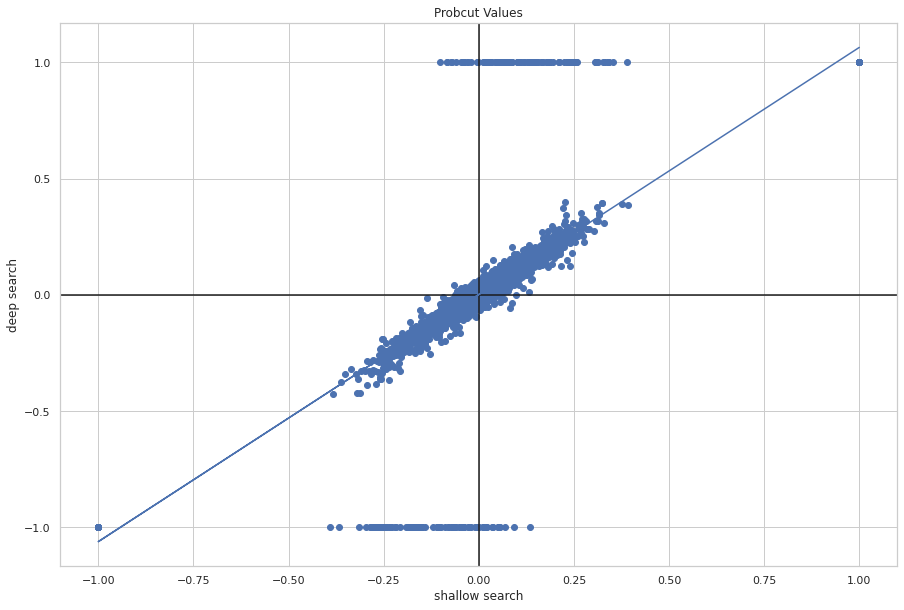
\includegraphics[width=\textwidth]{probcut_all_depths}
    \caption{Probcut Datenpunkte}
    \label{fig:probcut_all_depths}
\end{figure}

Wie zu erwarten, ist eine klare lineare Abhängigkeit zu erkennen, welche
durch die ebenfalls dargestellte Regressionsgerade hervorgehoben wird.
Die Ausreißer bei Deep Depth Werten von \(1\) und \(-1\) entstehen
dadurch, dass in diesen Spielzuständen, mit einer Tiefen Suche bereits
der Ausgang des Spiels bestimmt werden kann, während bei der Flachen
Suche noch die Heuristik verwendet wird. Theoretisch kann bereits hier
die Standardabeweichung ermittelt, und dann in ProbCut genutzt werden.
Bei zusätzlicher Betrachtung der Anzahl von Steinen auf dem Spielfeld
stellt sich jedoch heraus, dass die Standardabweichung stark davon
abhängt. Durch Einbeziehung der Steinzahl bei der Ermittleung der
Standardabweichung lässt sich also eine genauere Aussage über die
Standardabweichung machen.

Der folgende Code berechnet die Standardabweichung pro Anzahl Steine auf
dem Spielfeld. Dazu werden zunächst für jede Anzahl an Steinen aus den
Daten die passenden Werte extrahiert. Für diese Teilmengen wird jeweils
die Varianz mit \passthrough{\lstinline!numpy!} berechnet. Die
Standardabweichung ist dann die positive Wurzel aus der Varianz. Die
Anzahl an Steinen und die dazugehörige Standardabweichung werden in den
Feldern \passthrough{\lstinline!x!} und \passthrough{\lstinline!y!}
gespeichert.

\begin{lstlisting}[language=Python]
x = np.empty(0)
y = np.empty(0)

for i in range(5, 64):
    shallow_c = shallow[moves == i]
    deep_c = deep[moves == i]
    variance = np.var(np.stack([shallow_c, deep_c], axis=1))
    x = np.append(x, i)
    y = np.append(y, math.sqrt(variance))
\end{lstlisting}

Im Anschluss werden diese Daten visualisiert, um zu beurteilen, wie die
Standardabweichung durch eine geschlossene Formel angenähert werden
kann. Der Scatterplot kann in \autoref{fig:probcut_sigma_by_disccount}
betrachtet werden.

\begin{lstlisting}[language=Python]
plt.figure(figsize=(15, 10))
sns.set(style='whitegrid')
plt.scatter(x, y)
plt.axhline(y=0.0, c='k')
plt.xlabel('number of disks on the board')
plt.ylabel('standard deviation')
plt.title('Standard Deviation')
plt.show()
\end{lstlisting}

\begin{figure}[H]
    \centering
    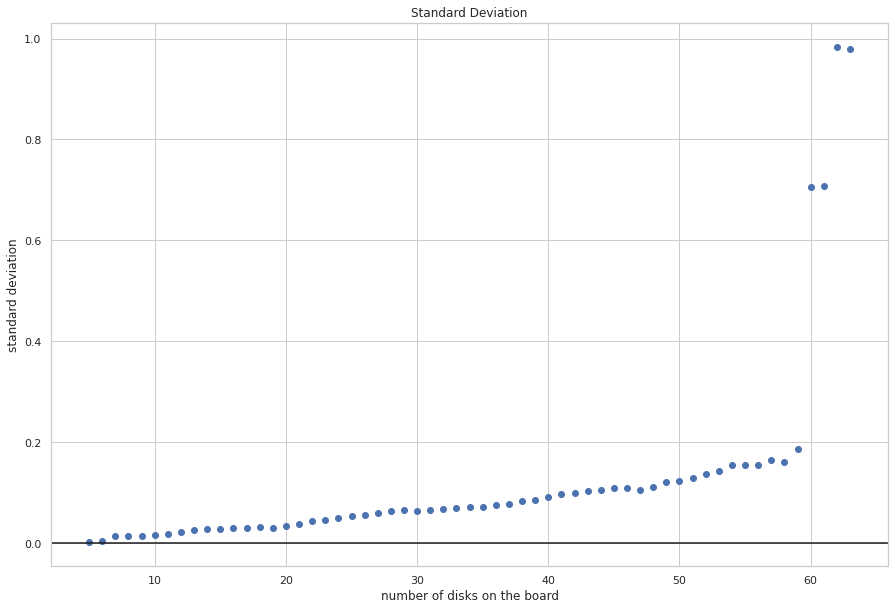
\includegraphics[width=\textwidth]{probcut_sigma_by_disccount}
    \caption{Probcut Standardabweichung abhängig von der Steinzahl}
    \label{fig:probcut_sigma_by_disccount}
\end{figure}

Bei der Betrachtung ergibt sich, dass im Bereich zwischen 5 und 58 Zügen
eine annähernd quadratische Abhängigkeit vorliegt. Daher wird dieser
Bereich mittels Polynomieller Regression angehähert und visualisiert.

Folgender Code berechnet das Regressionspolynom zweiten Gerades der
Standardabweichung in Abhängigkeit von der Anzahl der Steine auf dem
Spielfeld mit \passthrough{\lstinline!sklearn!} und stellt dieses, wie
in \autoref{fig:probcut_sigma_polynomial_regression} zu sehen, grafisch
dar.

\begin{lstlisting}[language=Python]
indices = np.argwhere(x <= 58)
xnew = x[indices]
ynew = y[indices][:,0]
polynomial_features= pp.PolynomialFeatures(degree=2)
xpoly = polynomial_features.fit_transform(xnew)

model = lm.LinearRegression()
model.fit(xpoly, ynew)

theta0 = model.intercept_
theta1, theta2, theta3 = model.coef_
a = np.arange(0.0, 60.0, 0.01)
b = theta0 + (theta1 + theta2) * a + theta3 * a**2

plt.figure(figsize=(15, 10))
sns.set(style='whitegrid')
plt.scatter(xnew, ynew)
plt.axhline(y=0.0, c='k')
plt.plot(a, b)
plt.xlabel('number of disks on the board')
plt.ylabel('standard deviation')
plt.title('Standard Deviation')
plt.show()
\end{lstlisting}

\begin{figure}[H]
    \centering
    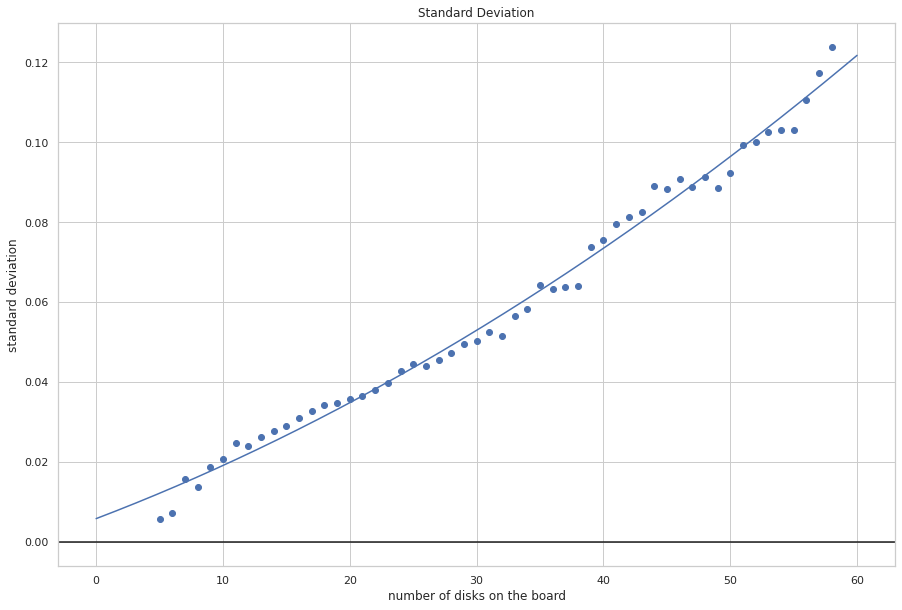
\includegraphics[width=\textwidth]{probcut_sigma_polynomial_regression}
    \caption{Annäherung der Standardabweichung durch Polynomielle Regression}
    \label{fig:probcut_sigma_polynomial_regression}
\end{figure}

Hier wird das Regressionspolynom ausgegeben, welches näherungsweise die
Standardabweichung in Abhängigkeit von der Anzahl an Spielsteinen auf
dem Spielfeld berechnet

\begin{lstlisting}[language=Python]
print(theta0, '+', theta1 + theta2, '* x +', theta3, '* x**2')
\end{lstlisting}

Die hier ausgegebenen Funktion wird in der ProbCut Implementierung zur
Bestimmung der Standardabweichung genutzt.

\hypertarget{gui-implementierung-othello_gui.ipynb}{%
\section{GUI Implementierung
(othello\_gui.ipynb)}\label{gui-implementierung-othello_gui.ipynb}}

\label{sec:gui}

\begin{lstlisting}[language=Python]
%%HTML
<style>
.container { width:100% }
</style>
\end{lstlisting}

Im folgenden Abschnitt wird eine Benutzeroberfläche für das Spiel
Othello implementiert. Diese ermöglicht das Anzeigen Spielfelds und das
Setzten von Steinen durch einen menschlichen Spieler per Mausklick.
Außerdem wird ein Einstellungsmenü implementiert, über welches das Spiel
und die KI Agenten konfiguriert werden können.

\hypertarget{importieren-der-externen-abhuxe4ngigkeiten}{%
\subsection{Importieren der externen
Abhängigkeiten}\label{importieren-der-externen-abhuxe4ngigkeiten}}

Die grafische Benutzeroberfläche verwendet zur Darstellung des
Spielzustandes, zum Anzeigen erweiterter Informationen sowie für die
Benutzerinteraktion die Bibliotheken \passthrough{\lstinline!ipycanvas!}
und \passthrough{\lstinline!ipywidgets!}. Diese können direkt im Jupyter
Notebook verwendet werden.

Zusätzlich werden aus dem Paket \passthrough{\lstinline!math!} der
Python Standardbibliothek die Variable \passthrough{\lstinline!pi!}
sowie die Funktion \passthrough{\lstinline!floor!} benötigt.

\begin{lstlisting}[language=Python]
import ipycanvas
import ipywidgets
import math
from ipywidgets import RadioButtons, HBox, VBox, IntSlider, Label
\end{lstlisting}

\hypertarget{konfiguration-der-gui}{%
\subsection{Konfiguration der GUI}\label{konfiguration-der-gui}}

Die Grafische Benutzeroberfläche unterstützt optional die Anzeige aller
möglichen Züge in der aktuellen Spielsituation, sowie die Darstellung
der Menge \passthrough{\lstinline!frontier!}, welche im
\autoref{sec:gamelogic} beschrieben wird. Ob diese Features verwendet
werden, wird im Folgenden mit den Konstanten
\passthrough{\lstinline!SHOW\_FRONTIER!} und
\passthrough{\lstinline!SHOW\_POSSIBLE\_MOVES!} konfiguriert.

\begin{lstlisting}[language=Python]
SHOW_FRONTIER = False
SHOW_POSSIBLE_MOVES = True
\end{lstlisting}

\hypertarget{canvas-initialisierung}{%
\subsection{Canvas Initialisierung}\label{canvas-initialisierung}}

Zunächst wird ein Canvas Objekt der Bibliothek
\passthrough{\lstinline!ipycanvas!} initialisiert, auf dem später das
Spielfeld dargestellt wird. Die Konstante
\passthrough{\lstinline!CELL\_SIZE!} beschreibt hierbei die Größe eines
einzelen Feldes in Pixeln auf dem Spielbrett, wohingegen
\passthrough{\lstinline!CANVAS\_SIZE!} die Größe des gesamten
Spielbretts angibt.

\begin{lstlisting}[language=Python]
CELL_SIZE = 60

CANVAS_SIZE = BOARD_SIZE * CELL_SIZE

canvas = ipycanvas.MultiCanvas(2, width=CANVAS_SIZE, height=CANVAS_SIZE)
canvas[0].fill_style = 'darkgreen'
canvas[0].stroke_style = 'black'
canvas[0].fill_rect(0, 0, CANVAS_SIZE, CANVAS_SIZE)
canvas[0].begin_path()
for i in range(BOARD_SIZE+1):
    pos = i * CELL_SIZE
    canvas[0].move_to(pos, 0)
    canvas[0].line_to(pos, CANVAS_SIZE)
    canvas[0].move_to(0, pos)
    canvas[0].line_to(CANVAS_SIZE, pos)
canvas[0].stroke()
\end{lstlisting}

\hypertarget{widget-initialisierung}{%
\subsection{Widget Initialisierung}\label{widget-initialisierung}}

Unter dem Spielfeld werden mit der Bibliothek
\passthrough{\lstinline!ipywidgets!} zusätzliche Informationen zum
aktuellen Spielzustand angezeigt. Diese werden mithilfe sogenannter
Widgets dargestellt, welche im Folgenden erzeugt werden.

Das \passthrough{\lstinline!score\_lbl!} Widget enthält die Steinzahl
beider Spieler im aktuellen Spielzustand.

\begin{lstlisting}[language=Python]
score_lbl = ipywidgets.widgets.Label()
\end{lstlisting}

Das \passthrough{\lstinline!turn\_lbl!} Widget nennt den Spieler, der
gerade am Zug ist.

\begin{lstlisting}[language=Python]
turn_lbl = ipywidgets.widgets.Label()
\end{lstlisting}

Das \passthrough{\lstinline!output!} Widget macht die Ausgabe mithilfe
von \passthrough{\lstinline!print()!}, sowie die Ausgabe von
Fehlermeldungen trotz der Verwendung von IPyWidgets und IPyCanvas
möglich.

\begin{lstlisting}[language=Python]
output = ipywidgets.widgets.Output()
\end{lstlisting}

Das Widget \passthrough{\lstinline!utility\_lbl!} dient der Anzeige der,
von den KI Spielern geschätzten, Nützlichkeit des Spielzustands.

\begin{lstlisting}[language=Python]
utility_lbl = ipywidgets.widgets.Label()
\end{lstlisting}

In der Funktion \passthrough{\lstinline!update\_output!} wird der
Spielzustand \passthrough{\lstinline!state!} auf den existierenden
Canvas gezeichnet.

\begin{lstlisting}[language=Python]
def update_output(state):
    with ipycanvas.hold_canvas(canvas):
        canvas[1].clear()
        for ((x, y), val) in np.ndenumerate(state.board):
            if val == NONE:
                continue
            elif val == BLACK:
                canvas[1].fill_style = 'black'
            else:
                canvas[1].fill_style = 'white'
            canvas[1].fill_arc((x + 0.5) * CELL_SIZE, (y + 0.5)
                               * CELL_SIZE, CELL_SIZE / 2.2, 0, 2 * math.pi)

        if state.last_move != None:
            (x, y) = state.last_move
            canvas[1].stroke_style = 'red'
            canvas[1].line_width = 2
            canvas[1].stroke_arc((x + 0.5) * CELL_SIZE, (y + 0.5)
                               * CELL_SIZE, CELL_SIZE / 2.2, 0, 2 * math.pi)

        if SHOW_FRONTIER:
            for (x, y) in state.frontier:
                canvas[1].fill_style = 'gray'
                canvas[1].fill_arc((x + 0.5) * CELL_SIZE, (y + 0.5)
                                   * CELL_SIZE, CELL_SIZE / 6, 0, 2 * math.pi)

        if SHOW_POSSIBLE_MOVES:
            for (x, y) in get_possible_moves(state, state.turn):
                if state.turn == BLACK:
                    canvas[1].fill_style = 'black'
                else:
                    canvas[1].fill_style = 'white'
                canvas[1].fill_arc((x + 0.5) * CELL_SIZE, (y + 0.5)
                                   * CELL_SIZE, CELL_SIZE / 6, 0, 2 * math.pi)

    b_score = count_disks(state, BLACK)
    w_score = count_disks(state, WHITE)
    score_lbl.value = f'Black Player : {b_score} White Player : {w_score}'
    b_util = utilities[BLACK]
    w_util = utilities[WHITE]
    utility_lbl.value = f'Utility: Black: {b_util} / White: {w_util}'
    if state.game_over:
        turn_lbl.value = f'{get_player_string(get_utility(state))} wins'
    else:
        turn_lbl.value = f'{get_player_string(state.turn)}s Move'
\end{lstlisting}

Die Funktion \passthrough{\lstinline!display\_board!} stellt den durch
\passthrough{\lstinline!state!} angegebenen Spielzustand dar, indem
zunächst der Canvas per \passthrough{\lstinline!update\_output!}
aktualisiert, und dann zusammen mit den Status-Widgets angezeigt wird.

\begin{lstlisting}[language=Python]
def display_board(state):
    output.clear_output()
    update_output(state)
    display(canvas)
    display(score_lbl)
    display(turn_lbl)
    display(utility_lbl)
    display(output)
\end{lstlisting}

Für menschliche Spieler muss festgestellt werden, ob auf das Spielfeld
geklickt wurde. Dies geschieht in der Callback Funktion
\passthrough{\lstinline!mouse\_down!}, welche die x und y Koordinate des
Mausklicks relativ zum Canvas erhält. Auf Basis dieser Position wird,
falls möglich, ein Zug auf das angeklickte Feld gemacht. Die Funktion
wird durch den Aufruf von \passthrough{\lstinline!on\_mouse\_down!} auf
dem IPyCanvas als Callback Funktion registriert.

\begin{lstlisting}[language=Python]
def mouse_down(x_px, y_px):
    global state
    with output:
        if not state.game_over:
            x = math.floor(x_px / CELL_SIZE)
            y = math.floor(y_px / CELL_SIZE)
            try:
                state = make_move(state, (x, y))
            except InvalidMoveException:
                print('Invalid Move')
            update_output(state)
            try:
                next_move(state)
            except KeyboardInterrupt:
                pass

canvas[1].on_mouse_down(mouse_down)
\end{lstlisting}

\hypertarget{spieleinstellungen}{%
\subsection{Spieleinstellungen}\label{spieleinstellungen}}

Hier wird durch Nutzung von \passthrough{\lstinline!ipywidgets!} eine
Benutzerschnittstelle erzeugt, über die für beide Spieler Einstellungen
vorgenommen werden können. So kann zum Beispiel festelegt werden, ob ein
Spieler vom Nutzer, oder von einem KI-Agenten kontrolliert werden soll,
und Parameter der KI angepasst werden.

\begin{lstlisting}[language=Python]
algorithms = { 'Menschlicher Spieler': None,
               'ProbCut': probcut,
               'Alpha-Beta': alphabeta,
               'Minimax': minimax,
               'Zufällig': random_ai }
modes = { 'Feste Tiefe': ai_make_move,
          'Iterative Vertiefung': ai_make_move_id,
          'Zeitbegrenzte Vertiefung': ai_make_move_id_timelimited }
heuristics = { 'Cowthello': cowthello_heuristic,
               'Cowthello+': cowthello_safe_heuristic,
               'Mobilität': mobility_heuristic,
               'Kombiniert': combined_heuristic }
black_algorithm = RadioButtons(
    options=algorithms.keys(),
    value='Menschlicher Spieler',
    description='Schwarz:'
)
black_heuristic = RadioButtons(
    options=heuristics.keys(),
    value='Kombiniert'
)
black_mode = RadioButtons(
    options=modes.keys(),
    value='Zeitbegrenzte Vertiefung'
)
black_depth = IntSlider(value=5, min=1, max=10, description='Suchtiefe:')
black_timelimit = IntSlider(value=30, min=1, max=120, description='Zeitlimit:')
black_ints = VBox([black_depth, black_timelimit])
black_config = HBox([black_algorithm, black_mode, black_heuristic, black_ints])

white_algorithm = RadioButtons(
    options=algorithms.keys(),
    value='ProbCut',
    description='Weiß:'
)
white_heuristic = RadioButtons(
    options=heuristics.keys(),
    value='Kombiniert'
)
white_mode = RadioButtons(
    options=modes.keys(),
    value='Zeitbegrenzte Vertiefung'
)
white_depth = IntSlider(value=5, min=1, max=10, description='Suchtiefe:')
white_timelimit = IntSlider(value=30, min=1, max=120, description='Zeitlimit:')
white_ints = VBox([white_depth, white_timelimit])
white_config = HBox([white_algorithm, white_mode, white_heuristic, white_ints])
settings = ipywidgets.VBox([black_config, white_config])
\end{lstlisting}

Die Funktion \passthrough{\lstinline!configure\_settings!} dient der
Anzeige des Konfigurationsmenüs.

\begin{lstlisting}[language=Python]
def configure_settings():
    display(settings)
\end{lstlisting}

Die Funktion \passthrough{\lstinline!get\_settings!} liefert die über
das Konfigurationsmenü getätigte Konfiguration als Dictionary zurück.
Dies wird später im Frontend verwendet.

\begin{lstlisting}[language=Python]
def get_settings():
    return { BLACK: { 'heuristic': heuristics[black_heuristic.value],
                      'algorithm': algorithms[black_algorithm.value],
                      'depth': black_depth.value,
                      'timelimit': black_timelimit.value,
                      'mode': modes[black_mode.value] },
             WHITE: { 'heuristic': heuristics[white_heuristic.value],
                      'algorithm': algorithms[white_algorithm.value],
                      'depth': white_depth.value,
                      'timelimit': white_timelimit.value,
                      'mode': modes[white_mode.value] }}
\end{lstlisting}

\begin{lstlisting}[language=Python]
%%HTML
<style>
.container { width:100% }
</style>
\end{lstlisting}

\hypertarget{othello-frontend-othello.ipynb}{%
\section{Othello Frontend
(othello.ipynb)}\label{othello-frontend-othello.ipynb}}

\begin{lstlisting}[language=Python]
%run othello_ai.ipynb
%run othello_gui.ipynb
\end{lstlisting}

\begin{lstlisting}[language=Python]
import time
\end{lstlisting}

\hypertarget{applikation-starten}{%
\subsubsection{Applikation Starten}\label{applikation-starten}}

Im folgenden wird für beide Spieler die zu verwendende Künstliche
Intelligenz, sowie die jeweils angewandte Heuristik festgelegt. Ein Wert
von \passthrough{\lstinline!None!} bei der KI steht hierbei für einen
menschlichen Spieler. Die KIs und Heuristiken werden jeweils in einem
Dictionary gespeicher, sodass mit Spieler als Index auf die
entsprechende KI oder Heuristik zugegriffen werden kann.

\begin{lstlisting}[language=Python]
configure_settings()
\end{lstlisting}

Folgender Code dient zum Starten der interaktiven Applikation. Die
Funktion \passthrough{\lstinline!next\_move!} wird für jeden Spielzug
ausgeführt. Sie wird zu Beginn einmal aufgerufen. Wenn eine KI spielt,
wird die Funktion rekursiv für den nächsten Zug aufgerufen. Wenn der
Spieler menschlich ist, muss die Ausführung unterbrochen werden, da auf
das Aufrufen eines Callbacks durch einen Klick gewartet werden muss. Im
Callback wird auch die Funktion \passthrough{\lstinline!next\_move!} für
den nächsten Zug aufgerufen.

\begin{lstlisting}[language=Python]
state = GameState()
display_board(state)
settings = get_settings()

def next_move(old_state):
    global state
    # Check if/which AI is playing
    ai = settings[state.turn]['algorithm']
    if ai is not None:
        time.sleep(0.2)
        make_move = settings[old_state.turn]['mode']
        depth = settings[state.turn]['depth']
        timelim = settings[state.turn]['timelimit']
        heuristic = settings[old_state.turn]['heuristic']
        intval = timelim if make_move == ai_make_move_id_timelimited else depth
        print(intval)
        state = make_move(ai, old_state, intval, heuristic)
        update_output(state)
        if not state.game_over:
            next_move(state)
try:
    next_move(state)
except KeyboardInterrupt:
    pass
\end{lstlisting}

